\documentclass[tikz,border=10pt]{standalone}
\begin{document}
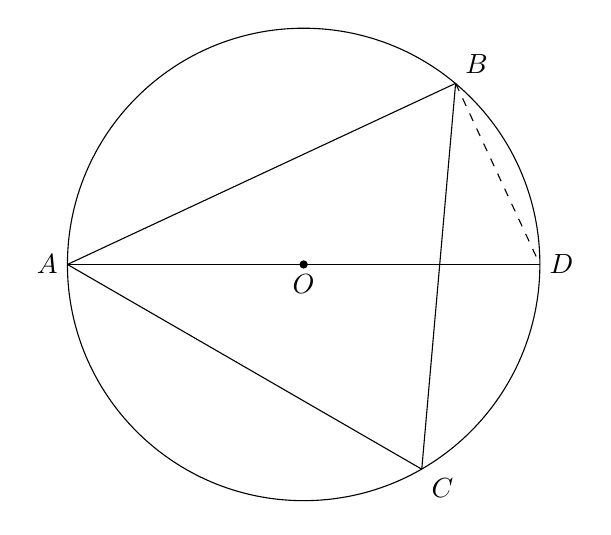
\begin{tikzpicture}
  \coordinate (A) at (-3,0);
  \coordinate (B) at (1.93,2.30);
  \coordinate (C) at (1.50,-2.60);
  \coordinate (D) at (3,0);
  \coordinate (O) at (0,0);

  \draw (O) circle (3);
  \draw (A) -- (D);
  \draw (A) -- (B);
  \draw (A) -- (C);
  \draw (B) -- (C);
  \draw[dashed] (B) -- (D);
  
  \fill (O) circle (1.5pt);

  \node[left] at (A) {$A$};
  \node[above right] at (B) {$B$};
  \node[below right] at (C) {$C$};
  \node[right] at (D) {$D$};
  \node[below] at (O) {$O$};
\end{tikzpicture}
\end{document}
